%%%%%%%%%%%%%%%%%%%%%%%%%%%%%%%%%%%%%%%%%%%%%%%%%%%%%%%%%%%%%%%%%%%%%%
% Lớp 12 | Tọa độ của véc-tơ trong không gian | Véc-tơ và các phép toán véc-tơ trong không gian (chưa tọa độ hóa)
% Dạng 2H2?1-2: Tổng, hiệu, tích một số với véc-tơ
% Số câu: 28  (sinh tự động bởi tach_cau.py; từ nay thầy sửa trực tiếp file này)
%%%%%%%%%%%%%%%%%%%%%%%%%%%%%%%%%%%%%%%%%%%%%%%%%%%%%%%%%%%%%%%%%%%%%%

%%%%%%%%%%%%%%%% TRẮC NGHIỆM 4 PHƯƠNG ÁN %%%%%%%%%%%%%%%%

% nguồn: Lop_12_Hinh_hoc_Chuong_2
\begin{ex}%[2H2N1-2]%[ma:e3be9366]
	\immini{Cho tứ  diện $ABCD$. Gọi $M$, $N$ lần lượt là trung điểm của $BC$, $CD$. Gọi $G$ là trọng tâm của tam giác $BCD$.}
	{\begin{tikzpicture}[line join=round,line cap=round,scale=0.8]
		\coordinate (B)  at (0,0);
		\coordinate  (D) at (6,0);
		\coordinate (C)  at (2,-2);
		\coordinate (A) at  ($(B)+(2,4)$);
		\coordinate (M)  at ($(C)!0.5!(B)$);
		\coordinate (N) at ($(C)!0.5!(D)$); 
		\coordinate (G)  at ($(B)!2/3!(N)$);
		\draw[->]  (A)--(B);
		 \draw[->] (A)--(D); \draw[->] (A)--(G);
		 \draw (B)--(C)--(D)
			 (A)--(C);
		\draw[dashed,thin](D)--(B)--(N) 
			(D)--(M); 
		\foreach \i/\g in {A/90,B/180,C/-90,D/-90,M/210,N/-30,G/-90}{\draw[fill=white](\i)  circle (1pt)
			($(\i)+(\g:3mm)$)  node[scale=.7]{$\i$};}
	\end{tikzpicture}
	 }
	Khẳng định  nào sau đây đúng?
	\choice 
		{$\overrightarrow{GA}+\overrightarrow{GB}=\overrightarrow{0}$} 
		 {$\overrightarrow{GM}+\overrightarrow{GN}=\overrightarrow{0}$}
		{$\overrightarrow{GA}+\overrightarrow{GB}+\overrightarrow{GC}=\overrightarrow{0}$} 
		{\True $\overrightarrow{GB}+\overrightarrow{GC}+\overrightarrow{GD}=\overrightarrow{0}$} 
	\loigiai{ 
		Do $G$ là  trọng tâm của tam giác $BCD$ nên ta có $\overrightarrow{GB}+\overrightarrow{GC}+\overrightarrow{GD}=\overrightarrow{0}$.
	} 
\end{ex}

% nguồn: Lop_12_Hinh_hoc_Chuong_2
\begin{ex}%[2H2N1-2]%[ma:e3282039]
	Cho hình hộp  $A B C D.A'B'C'D'$ có $\overrightarrow{A B}=\vec{a}$, $\overrightarrow{A D}=\vec{b}$, $\overrightarrow{AA'}=\vec{c}$. Khẳng định nào sau đây là đúng?
	\choice 
		 {\True $\overrightarrow{BD'}=-\vec{a}+\vec{b}+\vec{c}$}
		 {$\overrightarrow{BD'}=-\vec{a}-\vec{b}+\vec{c}$}
		{$\overrightarrow{BD'}=\vec{a}+\vec{b}+\vec{c}$} 
		 {$\overrightarrow{BD'}=\vec{a}-\vec{b}+\vec{c}$}
	 \loigiai{
		Áp  dụng quy tắc hình hộp, ta có $\overrightarrow{BD'}=\overrightarrow{B A}+\overrightarrow{B C}+\overrightarrow{BB'}=-\overrightarrow{A B}+\overrightarrow{B C}+\overrightarrow{BB'}=-\vec{a}+\vec{b}+\vec{c}$
	} 
\end{ex}

% nguồn: Lop_12_Hinh_hoc_Chuong_2
\begin{ex}%[2H2N1-2]%[ma:19a818c7]
	Trong không gian  $Oxyz$, cho các vectơ $\vec{a}=(2;-1; 3)$, $\vec{b}=(1; 3;-2)$. Tìm tọa độ của vectơ $\vec{c}=\vec{a} -2\vec{b}$.
	\choice 
		 {$\vec{c}=(0;-7;-7)$}
		 {\True $\vec{c}=(0;-7; 7)$}
		 {$\vec{c}=(0; 7; 7)$}
		{$\vec{c}=(4;-7;  7)$}
	\loigiai{ 
		 Ta có $\vec{c}=\vec{a} -2\vec{b}=(2-2;-1-6; 3+4)=(0;-7; 7)$.
	} 
\end{ex}

% nguồn: Lop_12_Hinh_hoc_Chuong_2
\begin{ex}%[2H2N1-2]%[ma:eb789c6e]
	 \immini{
	Cho hình hộp $ABCD.A_1B_1C_1D_1$. Véc-tơ nào dưới đây là véc-tơ đối  của $\overrightarrow{AB}$?
	 \choice
		{$\overrightarrow{BC}$} 
		 {$\overrightarrow{A_{1}B_{1}}$}
		{\True  $\overrightarrow{C_{1}D_{1}}$}
		{$\overrightarrow{DC}$} 
		} 
		 {
		\begin{tikzpicture}[scale=1,font=\footnotesize,line join=round,line cap=round,>=stealth]
				\path  (0,0) coordinate (A)
					(1,-1)  coordinate (B)
					(3,0)  coordinate (D)
					($(B)+(D)-(A)$)  coordinate (C);
				\foreach \x  in {A,B,C,D} \path (\x)+(1,3) coordinate (\x_1);
				\draw  (A)--(B)--(C)--(C_1)--(D_1)--(A_1)--cycle (A_1)--(B_1)--(C_1)
					(B_1)--(B) 
					 (C_1)--(C);
				\draw[dashed] (A)--(D)--(D_1) 
					(D)--(C); 
				\foreach \p/\r in {A/180,A_1/180,B/-90,B_1/60,D/0,D_1/90,C/0,C_1/0} 
				\fill  (\p) circle (1.5pt) node[shift={(\r:3mm)}]{$\p$};
			\end{tikzpicture}
		 }
	 \loigiai{
	Véc-tơ đối của $\overrightarrow{AB}$ là $\overrightarrow{C_{1}D_{1}}$.} 
\end{ex}

% nguồn: Lop_12_Hinh_hoc_Chuong_2
\begin{ex}%[2H2H1-2]%[ma:da938887]
	Cho hình chóp $S.ABCD$ có đáy $ABCD$  là hình bình hành. Đặt $\overrightarrow{SA}=\overrightarrow{a}$, $\overrightarrow{SB}=\overrightarrow{b}$, $\overrightarrow{SC}=\overrightarrow{c}$, $\overrightarrow{SD}=\overrightarrow{d}$. Khẳng định nào dưới đây là đúng?
	\choice 
		{\True  $\overrightarrow{a}+\overrightarrow{c}=\overrightarrow{b}+\overrightarrow{d}$}
		 {$\overrightarrow{a}+\overrightarrow{b}+\overrightarrow{c}+\overrightarrow{d}=\overrightarrow{0}$}
		 {$\overrightarrow{a}+\overrightarrow{d}=\overrightarrow{b}+\overrightarrow{c}$}
		 {$\overrightarrow{a}+\overrightarrow{b}=\overrightarrow{c}+\overrightarrow{d}$}
	 \loigiai{
	 \immini{
		Gọi $O$ là tâm hình  bình hành $ABCD$, suy ra\\
		 $\heva{&\overrightarrow{SA}+\overrightarrow{SC}=2\overrightarrow{SO}=\overrightarrow{a}+\overrightarrow{c}\\
		&\overrightarrow{SB}+\overrightarrow{SD}=2\overrightarrow{SO}=\overrightarrow{b}+\overrightarrow{d}}\Rightarrow\overrightarrow{a}+\overrightarrow{c}=\overrightarrow{b}+\overrightarrow{d}$. 
		}{ 
		\begin{tikzpicture}[line join=round,line cap=round,font=\footnotesize,scale=1,>=stealth]
				 \def \r{2.5}
				\path 
					(0,0) coordinate (A) 
					(80:0.8*\r)  coordinate (S)
					 (0:\r) coordinate (D)
					(220:0.6*\r) coordinate (B) 
					 ($(B)+(D)$) coordinate (C)
					 ($(A)!0.5!(C)$) coordinate (O);
				\draw  (S)--(B)--(C)--(D)--(S)--(B)
					(S)--(C); 
				\draw[dashed] (B)--(A)--(D) 
					 (S)--(O)
					 (B)--(D)
					 (S)--(A)--(C);
				\foreach \x/\g  in {S/90,A/180,B/180,C/-80,D/0,O/-90}\fill (\x) circle (1pt)+(\g:.3) node{$\x$};
			\end{tikzpicture}
		} 
	} 
\end{ex}

% nguồn: Lop_12_Hinh_hoc_Chuong_2
\begin{ex}%[2H2H1-2]%[ma:e13f2700]
	Cho hình chóp $S.ABCD$ có đáy là hình bình hành tâm $O$. Tính  tổng $\overrightarrow{SA}+\overrightarrow{SB}+\overrightarrow{SC}+\overrightarrow{SD}$.
	\choice 
		 {\True $4\overrightarrow{SO}$}
		{$\overrightarrow{SO}$} 
		{$\overrightarrow{0}$} 
		 {$2\overrightarrow{SO}$}
	\loigiai{ 
		\begin{center}
			\begin{tikzpicture}[scale=0.7,font=\footnotesize,line join=round,line cap=round,>=stealth]
					 \coordinate (A) at (0,0);
					 \coordinate (B) at (-2,-2);
					\coordinate  (D) at (5,0);
					\coordinate (C) at ($(B)+(D)-(A)$); 
					 \coordinate (O) at ($(A)!0.5!(C)$);
					 \coordinate (S) at ($(O)+(0,5)$);
					\draw  (S)--(B)
						 (S)--(C)--(D)--(S)
						 (B)--(C);
					\draw[dashed]  (C)--(A)--(B)
						 (C)--(D)
						(S)--(A)--(D)--(B) 
						 (S)--(O);
					 \foreach \i/\g in {S/90,A/180,B/-90,C/-90,D/0,O/-90}{\draw (\i) circle (1.5pt)
						($(\i)+(\g:3mm)$)  node[scale=1]{$\i$};}
				\end{tikzpicture}
		\end{center}
		Ta  có $\overrightarrow{SA}+\overrightarrow{SB}+\overrightarrow{SC}+\overrightarrow{SD}=( \overrightarrow{SA}+\overrightarrow{SC})+( \overrightarrow{SB}+\overrightarrow{SD})=2\overrightarrow{SO}+2\overrightarrow{SO}=4\overrightarrow{SO}$.
	} 
\end{ex}

% nguồn: Lop_12_Hinh_hoc_Chuong_2
\begin{ex}%[2H2H1-2]%[ma:509b7ff9]
	Cho hình lăng trụ $ABC.A'B'C'$. Đặt $\overrightarrow{AA'}=\overrightarrow{a}$, $\overrightarrow{AB}=\overrightarrow{b}$, $\overrightarrow{AC}=\overrightarrow{c}$. Gọi $G'$ là trọng tâm của tam giác $A'B'C'$. Véctơ $\overrightarrow{A{G}'}$ bằng 
	\choice 
		{$\dfrac{1}{3}\left(\overrightarrow{a}+3\overrightarrow{b}+\overrightarrow{c}\right)$} 
		 {\True $\dfrac{1}{3}\left(3\overrightarrow{a}+\overrightarrow{b}+\overrightarrow{c}\right)$}
		{$\dfrac{1}{3}\left(\overrightarrow{a}+\overrightarrow{b}+3\overrightarrow{c}\right)$} 
		 {$\dfrac{1}{3}\left(\overrightarrow{a}+\overrightarrow{b}+\overrightarrow{c}\right)$}
	\loigiai{ 
	\immini{ 
		 Gọi $I$ là trung điểm $B'C'$.\\
		Vì $G'$ là trọng  tâm tam giác $A'B'C'\Rightarrow\overrightarrow{A'G'}=\dfrac{2}{3}\overrightarrow{A'I}$.\\
		Mặt khác 
		\begin{eqnarray*}
			 \overrightarrow{AG'}&=&\overrightarrow{AA'}+\overrightarrow{A'G'}=\overrightarrow{AA'}+\dfrac{2}{3}\overrightarrow{A'I}=\overrightarrow{AA'}+\dfrac{1}{3}\left(\overrightarrow{A'B'}+\overrightarrow{A'C'}\right)\\
			&=&\overrightarrow{AA'}+\dfrac{1}{3}\left(\overrightarrow{AB}+\overrightarrow{AC}\right)=\dfrac{1}{3}\left(3\overrightarrow{AA'}+\overrightarrow{AB}+\overrightarrow{AC}\right)\\ 
			 &=&\dfrac{1}{3}\left(3\overrightarrow{a}+\overrightarrow{b}+\overrightarrow{c}\right).
		\end{eqnarray*}
		}{ 
		\begin{tikzpicture}[line join=round,line cap=round,font=\footnotesize,scale=1,>=stealth]
				 \def \r{3}
				\path 
					(0,0) coordinate  (A)
					(80:0.8*\r) coordinate  (A')
					(0:\r) coordinate  (B)
					 (-40:0.5*\r) coordinate (C)
					($(A')+(B)$)  coordinate (B')
					($(A')+(C)$)  coordinate (C')
					($(C')!0.5!(B')$)  coordinate (I)
					($(A')!2/3!(I)$) coordinate  (G');
				\draw (A')--(A)--(C)--(B)--(B')--(A')--(C')--(C) 
					 (C')--(B')
					(A')--(I); 
				\draw[dashed] (A)--(B); 
				\foreach \x/\g in {A/180,B/-50,C/-90,A'/90,B'/90,C'/-30,G'/-100,I/-80}\fill (\x) circle  (1pt)+(\g:.3) node{$\x$};
			\end{tikzpicture}
		 }
	 }
\end{ex}

% nguồn: Lop_12_Hinh_hoc_Chuong_2
\begin{ex}%[2H2H1-2]%[ma:4455d72c]
	Cho hình tứ diện $ABCD$ có trọng tâm $G$. Mệnh đề nào sau đây \textbf{sai}? 
	 \choice
		{$\overrightarrow{GA}+\overrightarrow{GB}+\overrightarrow{GC}+\overrightarrow{GD}=\overrightarrow{0}$} 
		{$\overrightarrow{OG}=\dfrac{1}{4}\left(\overrightarrow{OA}+\overrightarrow{OB}+\overrightarrow{OC}+\overrightarrow{OD}\right)$} 
		{\True  $\overrightarrow{AG}=\dfrac{1}{3}\left(\overrightarrow{AB}+\overrightarrow{AC}+\overrightarrow{AD}\right)$}
		{$\overrightarrow{AG}=\dfrac{1}{4}\left(\overrightarrow{AB}+\overrightarrow{AC}+\overrightarrow{AD}\right)$} 
	 \loigiai{
		Có $G$ là trọng tâm của tứ diện $ABCD$ nên 
		\begin{align*}
			\overrightarrow{GA}+\overrightarrow{GB}+\overrightarrow{GC}+\overrightarrow{GD}=\overrightarrow{0}&\Leftrightarrow  4\overrightarrow{GA}+\overrightarrow{AB}+\overrightarrow{AC}+\overrightarrow{AD}=\overrightarrow{0}\\ &\Leftrightarrow\overrightarrow{AG}=\dfrac{1}{4}\left(\overrightarrow{AB}+\overrightarrow{AC}+\overrightarrow{AD}\right).
		\end{align*}
	 }
\end{ex}

% nguồn: Lop_12_Hinh_hoc_Chuong_2
\begin{ex}%[2H2H1-2]%[ma:2bb2c478]
	Cho hình lăng trụ tam giác $ABC.A'B'C'$. Đặt $\overrightarrow{AA'}=\overrightarrow{a}$, $\overrightarrow{AB}=\overrightarrow{b}$, $\overrightarrow{AC}=\overrightarrow{c}$, $\overrightarrow{BD}=\overrightarrow{d}$.  Khẳng định nào sau đây là đúng?
	\choice 
		 {$\overrightarrow{a}=\overrightarrow{b}+\overrightarrow{c}$}
		 {$\overrightarrow{a}+\overrightarrow{b}+\overrightarrow{c}+\overrightarrow{d}=\overrightarrow{0}$}
		{\True $\overrightarrow{b}-\overrightarrow{c}+\overrightarrow{d}=\overrightarrow{0}$} 
		{$\overrightarrow{a}+\overrightarrow{b}+\overrightarrow{c}=\overrightarrow{d}$} 
	 \loigiai{
	 \immini{
		Ta  có $\overrightarrow{BC}=\overrightarrow{AC}-\overrightarrow{AB}\Leftrightarrow\overrightarrow{d}=\overrightarrow{c}-\overrightarrow{b}\Leftrightarrow\overrightarrow{b}-\overrightarrow{c}+\overrightarrow{d}=\overrightarrow{0}$.
		}{ 
		\begin{tikzpicture}[line join=round,line cap=round,font=\footnotesize,scale=1,>=stealth]
				 \def \r{3}
				 \path
					(0,0)  coordinate (A)
					(80:0.6*\r) coordinate  (A')
					 (0:\r) coordinate (B)
					(-40:0.5*\r) coordinate  (C)
					 ($(A')+(B)$) coordinate (B')
					 ($(A')+(C)$) coordinate (C');
				\draw (A')--(A)--(C)--(B)--(B')--(A')--(C')--(C) 
					 (C')--(B');
				\draw[dashed]  (A)--(B);
				\foreach \x/\g in {A/180,B/-50,C/-90,A'/90,B'/90,C'/-30}\fill (\x) circle (1pt)+(\g:.3)  node{$\x$};
			\end{tikzpicture}
		} 
	 }
\end{ex}

% nguồn: Lop_12_Hinh_hoc_Chuong_2
\begin{ex}%[2H2H1-2]%[ma:15782263]
	Cho  tứ diện $ABCD$ gọi $I$, $J$ lần lượt là trung điểm của $AB$ và $CD$. Đẳng thức nào \textbf{sai}?
	 \choice
		 {$\overrightarrow{IJ}=\dfrac{1}{2}\left(\overrightarrow{AC}+\overrightarrow{BD}\right)$}
		 {$\overrightarrow{IJ}=\dfrac{1}{2}\left(\overrightarrow{AD}+\overrightarrow{BC}\right)$}
		 {$\overrightarrow{IJ}=\dfrac{1}{2}\left(\overrightarrow{DC}+\overrightarrow{AD}+\overrightarrow{BD}\right)$}
		 {\True $\overrightarrow{IJ}=\dfrac{1}{2}\left(\overrightarrow{AB}+\overrightarrow{CD}\right)$}
	\loigiai{ 
		\begin{center}
			\begin{tikzpicture}[scale=1,font=\footnotesize,line join=round,line cap=round,>=stealth]
					 \path
						(0,0)  coordinate (B)
						 (1,3) coordinate (A)
						(5,0) coordinate (D) 
						(1.5,-1)  coordinate (C)
						 ($(B)!0.5!(A)$) coordinate (I)
						($(D)!0.5!(C)$) coordinate (J); 
					\draw  (A)--(B)--(C)--(A)--(D)--(C);
					\draw[dashed]  (I)--(J)
						(B)--(D); 
					\foreach \t/\g in {A/90,B/180,C/-90,D/0,I/170,J/-30}{ 
						\draw  (\t) circle (.5pt) node[shift={(\g:7pt)},font=\scriptsize]{$ \t $};
					 }
				\end{tikzpicture}
		\end{center}
		Ta có \begin{eqnarray*}\overrightarrow{IJ}&=&\overrightarrow{IA}+\overrightarrow{AJ}=-\dfrac{1}{2}\overrightarrow{AB}+\dfrac{1}{2}\left(\overrightarrow{AC}+\overrightarrow{AD}\right)\\
		&=&\dfrac{1}{2}\left(\overrightarrow{BC}+\overrightarrow{AD}\right)=\dfrac{1}{2}\left(\overrightarrow{AB}+\overrightarrow{BD}+\overrightarrow{CD}+\overrightarrow{DC}+\overrightarrow{BC}\right)\\ 
		 &=&\dfrac{1}{2}\left(\overrightarrow{AB}+\overrightarrow{CD}+2\overrightarrow{BC}\right).
	\end{eqnarray*}
	Vậy  đẳng thức \textbf{sai} là $\overrightarrow{IJ}=\dfrac{1}{2}\left(\overrightarrow{AB}+\overrightarrow{CD}\right)$.
} 
\end{ex}

% nguồn: Lop_12_Hinh_hoc_Chuong_2
\begin{ex}%[2H2H1-2]%[ma:7c35ce7e]
	 Cho tứ diện $ABCD$. Đặt $\overrightarrow{AB}=\overrightarrow{a}$, $\overrightarrow{AC}=\overrightarrow{b}$, $\overrightarrow{AD}=\overrightarrow{c}$. Gọi $G$ là trọng tâm tam giác $BCD$. Đẳng thức nào sau đây đúng?
	 \choice
		 {$\overrightarrow{AG}=\overrightarrow{a}+\overrightarrow{b}+\overrightarrow{c}$}
		 {\True $\overrightarrow{AG}=\dfrac{1}{3}\left(\overrightarrow{a}+\overrightarrow{b}+\overrightarrow{c}\right)$}
		 {$\overrightarrow{AG}=\dfrac{1}{2}\left(\overrightarrow{a}+\overrightarrow{b}+\overrightarrow{c}\right)$}
		{$\overrightarrow{AG}=\dfrac{1}{4}\left(\overrightarrow{a}+\overrightarrow{b}+\overrightarrow{c}\right)$} 
	\loigiai{ 
	\immini{ 
		Gọi $M$ là trung điểm của $CD$, suy ra  $\overrightarrow{BG}=\dfrac{2}{3}\overrightarrow{BM}$.\\
		Mặt  khác
		\begin{eqnarray*}
			\overrightarrow{AG}&=&\overrightarrow{AB}+\overrightarrow{BG}=\overrightarrow{AB}+\dfrac{2}{3}\overrightarrow{BM}=\overrightarrow{AB}+\dfrac{2}{3}\cdot\dfrac{1}{2}\left(\overrightarrow{BC}+\overrightarrow{BD}\right)\\ 
			 &=&\overrightarrow{AB}+\dfrac{1}{3}\left(\overrightarrow{AC}-\overrightarrow{AB}+\overrightarrow{AD}-\overrightarrow{AB}\right)=\dfrac{1}{3}\left(\overrightarrow{AB}+\overrightarrow{AC}+\overrightarrow{AD}\right)\\
			&=&\dfrac{1}{3}\left(\overrightarrow{a}+\overrightarrow{b}+\overrightarrow{c}\right). 
		\end{eqnarray*}
		}{ 
		\begin{tikzpicture}[line join=round,line cap=round,font=\footnotesize,scale=1,>=stealth]
				\def \r{3} 
				 \path
					(0,0)  coordinate (B)
					(0:\r)  coordinate (D)
					 (-40:0.5*\r) coordinate (C)
					(60:0.7*\r) coordinate  (A)
					($(C)!0.5!(D)$)  coordinate (M)
					 ($(B)!2/3!(M)$) coordinate (G);
				 \draw (A)--(B)--(C)--(D)--(A)--(C);
				\draw[dashed]  (B)--(D)
					(A)--(G) 
					 (B)--(M);
				\foreach \x/\g in {A/90,B/180,C/-90,D/0,G/-90,M/-20}\fill (\x) circle  (1pt)+(\g:.3) node{$\x$};
			\end{tikzpicture}
		 }
	} 
\end{ex}

% nguồn: Lop_12_Hinh_hoc_Chuong_2
\begin{ex}%[2H2H1-2]%[ma:9fd65ecf]
	Trong không gian $Oxyz$, cho hai điểm $A(1;2;0)$, $B(-1;3;5)$. Gọi $I(a;b;c)$ là điểm thỏa mãn $\overrightarrow{IA}+3\overrightarrow{IB}=\overrightarrow{0}$. Khi  đó, giá trị của biểu thức $a+2b+2c$ bằng
	\choice 
		{\True $\dfrac{25}{2}$} 
		{$-\dfrac{25}{2}$} 
		{$50$} 
		 {$\dfrac{27}{2}$}
	 \loigiai{
		Ta có 
		\begin{eqnarray*}
			&&\overrightarrow{IA}+3\overrightarrow{IB}=\overrightarrow{0}\\ 
			 &\Leftrightarrow&(1-a;2-b;-c)=(3+3a;3b-9;3c-15)\\
			&\Leftrightarrow&\heva{&1-a=3+3a\\&2-b=3b-9\\&-c=3c-15}\\ 
			 &\Leftrightarrow&\heva{&a=-\dfrac{1}{2}\\&b=\dfrac{11}{4}\\&c=\dfrac{15}{4}.}
		\end{eqnarray*}
		Vậy  $a+2b+2c=\dfrac{25}{2}$.
	} 
\end{ex}

% nguồn: Lop_12_Hinh_hoc_Chuong_2
\begin{ex}%[2H2H1-2]%[ma:9443ff44]
	Cho hình hộp $ABCD.A'B'C'D'$. Đặt $\overrightarrow{AB}=\overrightarrow{a}$,  $\overrightarrow{AD}=\overrightarrow{b}$, $\overrightarrow{AA'}=\overrightarrow{c}$. Phân tích vectơ $\overrightarrow{AC'}$ theo $\overrightarrow{a},\overrightarrow{b},\overrightarrow{c}$.
	 \choice
		 {$\overrightarrow{AC'}=-\overrightarrow{a}+\overrightarrow{b}+\overrightarrow{c}$}
		{$\overrightarrow{AC'}=\overrightarrow{a}+\overrightarrow{b}-\overrightarrow{c}$} 
		{\True  $\overrightarrow{AC'}=\overrightarrow{a}+\overrightarrow{b}+\overrightarrow{c}$}
		{$\overrightarrow{AC'}=\overrightarrow{a}-\overrightarrow{b}+\overrightarrow{c}$} 
	 \loigiai{
	\immini{ 
		Ta  có $\overrightarrow{AC'}=\overrightarrow{AA'}+\overrightarrow{AC}=\overrightarrow{AA'}+\overrightarrow{AB}+\overrightarrow{AD}=\overrightarrow{a}+\overrightarrow{b}+\overrightarrow{c}$.
		 }{
		\begin{tikzpicture}[line join=round,line cap=round,font=\footnotesize,scale=1,>=stealth]
				\def \r{2} 
				\path 
					 (0,0) coordinate (A)
					 (80:\r) coordinate (A')
					(0:\r)  coordinate (D)
					(230:0.6*\r) coordinate (B) 
					($(B)+(D)$)  coordinate (C)
					($(A')+(B)$) coordinate (B') 
					 ($(A')+(C)$) coordinate (C')
					($(A')+(D)$) coordinate (D'); 
				 \draw (B')--(B)--(C)--(D)--(D')--(A')--(B')--(C')--(D')
					(C)--(C') 
					 (A')--(C');
				 \draw[dashed] (B)--(A)--(D)
					 (A)--(A')
					(C')--(A)--(C); 
				 \foreach \x/\g in {A/-80,B/180,C/-80,D/0,A'/120,B'/180,C'/-20,D'/90}\fill (\x) circle (1pt)+(\g:.3) node{$\x$};
			\end{tikzpicture}
		 }
	} 
\end{ex}

% nguồn: Lop_12_Hinh_hoc_Chuong_2
\begin{ex}%[2H2H1-2]%[ma:e98b41c8]
	Cho hình lăng  trụ $ABC.A'B'C'$. Đặt $\overrightarrow{AA'}=\overrightarrow{a}$, $\overrightarrow{AB}=\overrightarrow{b}$, $\overrightarrow{AC}=\overrightarrow{c}$. Hãy biểu diễn vectơ $\overrightarrow{B'C}$ theo $\overrightarrow{a},\overrightarrow{b},\overrightarrow{c}$.
	\choice 
		 {$\overrightarrow{B'C}=\overrightarrow{a}+\overrightarrow{b}-\overrightarrow{c}$}
		{$\overrightarrow{B'C}=-\overrightarrow{a}+\overrightarrow{b}-\overrightarrow{c}$} 
		{$\overrightarrow{B'C}=\overrightarrow{a}+\overrightarrow{b}+\overrightarrow{c}$} 
		{\True $\overrightarrow{B'C}=-\overrightarrow{a}-\overrightarrow{b}+\overrightarrow{c}$} 
	 \loigiai{
	 \immini{
		Vì $BB'C'C$  là hình bình hành nên
		\begin{eqnarray*}
			 \overrightarrow{B'C}&=&\overrightarrow{B'C'}+\overrightarrow{B'B}=\overrightarrow{BC}-\overrightarrow{AA'}\\
			 &=&-\overrightarrow{AA'}+\overrightarrow{BA}+\overrightarrow{AC}=-\overrightarrow{AA'}-\overrightarrow{AB}+\overrightarrow{AC}\\
			&=&-\overrightarrow{a}-\overrightarrow{b}+\overrightarrow{c}. 
		\end{eqnarray*}
		}{ 
		\begin{tikzpicture}[line join=round,line cap=round,font=\footnotesize,scale=1,>=stealth]
				 \def \r{3}
				 \path
					(0,0) coordinate  (A)
					(80:0.8*\r) coordinate  (A')
					(0:\r) coordinate (B) 
					(-40:0.5*\r)  coordinate (C)
					($(A')+(B)$) coordinate  (B')
					($(A')+(C)$) coordinate  (C');
				 \draw (A')--(A)--(C)--(B)--(B')--(A')--(C')--(C)
					 (C')--(B')
					 (C)--(B');
				 \draw[dashed] (A)--(B);
				\foreach \x/\g in {A/180,B/-50,C/-90,A'/90,B'/90,C'/-30}\fill  (\x) circle (1pt)+(\g:.3) node{$\x$};
			\end{tikzpicture}
		} 
	 }
\end{ex}

% nguồn: Lop_12_Hinh_hoc_Chuong_2
\begin{ex}%[2H2H1-2]%[ma:84a58b66]
	 Cho hình lập phương $ABCD.A'B'C'D'$. Gọi $O$ là tâm của hình lập phương. Khẳng định nào sau đây là đúng?
	 \choice
		{$\overrightarrow{AO}=\dfrac{1}{3}\left(\overrightarrow{AB}+\overrightarrow{AD}+\overrightarrow{AA'}\right)$} 
		{\True $\overrightarrow{AO}=\dfrac{1}{2}\left(\overrightarrow{AB}+\overrightarrow{AD}+\overrightarrow{AA'}\right)$} 
		 {$\overrightarrow{AO}=\dfrac{1}{4}\left(\overrightarrow{AB}+\overrightarrow{AD}+\overrightarrow{AA'}\right)$}
		 {$\overrightarrow{AO}=\dfrac{2}{3}\left(\overrightarrow{AB}+\overrightarrow{AD}+\overrightarrow{AA'}\right)$}
	 \loigiai{
	\immini{ 
		Ta có  $\overrightarrow{AC'}=\overrightarrow{AB}+\overrightarrow{AD}+\overrightarrow{AA'}$.\\
		Mặt  khác $O$ là trung điểm $AC'$, suy ra\\
		 $\overrightarrow{AO}=\dfrac{1}{2}\overrightarrow{AC'}=\dfrac{1}{2}\left(\overrightarrow{AB}+\overrightarrow{AD}+\overrightarrow{AA'}\right)$.
		 }{
		\begin{tikzpicture}[line join=round,line cap=round,font=\footnotesize,scale=1,>=stealth]
				\def \r{2} 
				\path 
					(0,0) coordinate (A) 
					(90:\r) coordinate  (A')
					(0:\r)  coordinate (D)
					(230:0.6*\r) coordinate (B) 
					($(B)+(D)$) coordinate  (C)
					($(A')+(B)$) coordinate  (B')
					($(A')+(C)$) coordinate (C') 
					 ($(A')+(D)$) coordinate (D')
					($(A)!0.5!(C')$) coordinate (O); 
				 \draw (B')--(B)--(C)--(D)--(D')--(A')--(B')--(C')--(D')
					 (C)--(C');
				 \draw[dashed] (B)--(A)--(D)
					 (A)--(A')
					(C')--(A); 
				\foreach \x/\g in {A/-80,B/180,C/-80,D/0,A'/120,B'/180,C'/80,D'/90,O/-20}\fill (\x)  circle (1pt)+(\g:.3) node{$\x$};
			\end{tikzpicture}
		 }
	} 
\end{ex}

% nguồn: Lop_12_Hinh_hoc_Chuong_2
\begin{ex}%[2H2H1-2]%[ma:ac1badfd]
	Cho hình lăng trụ $ABC.A'B'C'$. Gọi $M$  là trung điểm của cạnh $BB'$. Đặt $\overrightarrow{CA}=\overrightarrow{a}$, $\overrightarrow{CB}=\overrightarrow{b}$, $\overrightarrow{AA'}=\overrightarrow{c}$. Khẳng định nào sau đây đúng?
	\choice 
		{$\overrightarrow{AM}=\overrightarrow{a}+\overrightarrow{c}-\dfrac{1}{2}\overrightarrow{b}$} 
		 {$\overrightarrow{AM}=\overrightarrow{b}+\overrightarrow{c}-\dfrac{1}{2}\overrightarrow{a}$}
		{\True $\overrightarrow{AM}=\overrightarrow{b}-\overrightarrow{a}+\dfrac{1}{2}\overrightarrow{c}$} 
		 {$\overrightarrow{AM}=\overrightarrow{a}-\overrightarrow{c}+\dfrac{1}{2}\overrightarrow{b}$}
	 \loigiai{
	 \immini{
		Vì $M$ là trung điểm  $BB'$ suy ra $\overrightarrow{BM}=\dfrac{1}{2}\overrightarrow{BB'}$.\\
		 Mặt khác
		\begin{eqnarray*}
			\overrightarrow{AM}&=&\overrightarrow{AB}+\overrightarrow{BM}=-\overrightarrow{BA}+\dfrac{1}{2}\overrightarrow{BB'}=-\overrightarrow{CA}+\overrightarrow{CB}+\dfrac{1}{2}BB'\\ 
			&=&-\overrightarrow{a}+\overrightarrow{b}+\dfrac{1}{2}\overrightarrow{c}. 
		\end{eqnarray*}
		 }{
		\begin{tikzpicture}[line join=round,line cap=round,font=\footnotesize,scale=1,>=stealth]
				\def \r{3} 
				\path 
					(0,0) coordinate (A) 
					(80:0.8*\r) coordinate  (A')
					(0:\r) coordinate  (B)
					(-40:0.5*\r) coordinate (C) 
					($(A')+(B)$) coordinate (B') 
					($(A')+(C)$) coordinate  (C')
					 ($(B)!0.5!(B')$) coordinate (M);
				 \draw (A')--(A)--(C)--(B)--(B')--(A')--(C')--(C)
					(C')--(B'); 
				 \draw[dashed] (M)--(A)--(B);
				\foreach \x/\g  in {A/180,B/-50,C/-90,A'/90,B'/90,C'/-30,M/-30}\fill (\x) circle (1pt)+(\g:.3) node{$\x$};
			\end{tikzpicture}
		 }
	 }
\end{ex}

% nguồn: Lop_12_Hinh_hoc_Chuong_2
\begin{ex}%[2H2H1-2]%[ma:f651046e]
	Cho tứ  diện $ABCD$. Đặt $\overrightarrow{AB}=\overrightarrow{a}$, $\overrightarrow{AC}=\overrightarrow{b}$, $\overrightarrow{AD}=\overrightarrow{c}$. Gọi $M$ là trung điểm của đoạn $BC$. Đẳng thức nào dưới đây đúng?
	\choice 
		 {\True $\overrightarrow{DM}=\dfrac{1}{2}\left(\overrightarrow{a}+\overrightarrow{b}-2\overrightarrow{c}\right)$}
		 {$\overrightarrow{DM}=\dfrac{1}{2}\left(\overrightarrow{a}+2\overrightarrow{b}-\overrightarrow{c}\right)$}
		{$\overrightarrow{DM}=\dfrac{1}{2}\left(\overrightarrow{a}-2\overrightarrow{b}+\overrightarrow{c}\right)$} 
		{$\overrightarrow{DM}=\dfrac{1}{2}\left(\overrightarrow{a}+2\overrightarrow{b}+\overrightarrow{c}\right)$} 
	\loigiai{ 
	\immini{ 
		Vì  $M$ là trung điểm của $BC$, suy ra $\overrightarrow{BM}=\dfrac{1}{2}\overrightarrow{BC}$.\\
		Mặt  khác
		\begin{eqnarray*}
			\overrightarrow{DM}&=&\overrightarrow{DA}+\overrightarrow{AB}+\overrightarrow{BM}=\overrightarrow{AB}-\overrightarrow{AD}+\dfrac{1}{2}\overrightarrow{BC}\\ 
			 &=&\overrightarrow{AB}-\overrightarrow{AD}+\dfrac{1}{2}\left(\overrightarrow{BA}+\overrightarrow{AC}\right)=\dfrac{1}{2}\overrightarrow{AB}+\dfrac{1}{2}\overrightarrow{AC}-\overrightarrow{AD}\\ &=&\dfrac{1}{2}\overrightarrow{a}+\dfrac{1}{2}\overrightarrow{b}-\overrightarrow{c}=\dfrac{1}{2}\left(\overrightarrow{a}+\overrightarrow{b}-2\overrightarrow{c}\right).
		\end{eqnarray*}
		 }{
		\begin{tikzpicture}[line join=round,line cap=round,font=\footnotesize,scale=1,>=stealth]
				\def \r{2.5} 
				 \path
					 (0,0) coordinate (B)
					(60:0.7*\r) coordinate  (A)
					 (0:\r) coordinate (D)
					(-40:0.5*\r) coordinate  (C)
					($(B)!0.5!(C)$)  coordinate (M);
				 \draw[-stealth](A)--(B);
				\draw[-stealth](A)--(C); 
				\draw[-stealth](A)--(D); 
				\draw  (B)--(C)--(D)
					 (A)--(M);
				 \draw[dashed] (B)--(D)
					 (M)--(D);
				\foreach \x/\g in {A/90,B/180,C/-90,D/0,M/-120}\fill (\x) circle  (1pt)+(\g:.3) node{$\x$};
			\end{tikzpicture}
		 }
	 }
\end{ex}

% nguồn: Lop_12_Hinh_hoc_Chuong_2
\begin{ex}%[2H2H1-2]%[ma:b48b3031]
	Cho tứ diện $ABCD$. Điểm $N$ xác định bởi đẳng thức  sau $\overrightarrow{AN}=\overrightarrow{AB}+\overrightarrow{AC}-\overrightarrow{AD}$. Mệnh đề nào đúng?
	\choice 
		{$N$ là trung điểm  $BD$}
		{$N$ là đỉnh hình bình hành  $BCDN$}
		{\True $N$ là đỉnh  hình bình hành $CDBN$}
		{$N\equiv  A$}
	\loigiai{ 
	 \immini{
		Ta có  $\overrightarrow{AN}=\overrightarrow{AB}+\overrightarrow{AC}-\overrightarrow{AD}\Leftrightarrow\overrightarrow{AN}-\overrightarrow{AB}=\overrightarrow{AC}-\overrightarrow{AD}\Leftrightarrow\overrightarrow{BN}=\overrightarrow{DC}$.\\
		Suy ra $N$ là đỉnh thứ tư  của hình bình hành $CDBN$.
		}{ 
		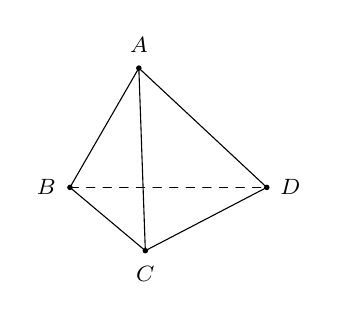
\begin{tikzpicture}[line join=round,line cap=round,font=\footnotesize,scale=1,>=stealth]
				\def \r{2.5} 
				 \path
					(0,0) coordinate (B) 
					(60:0.7*\r)  coordinate (A)
					(0:\r) coordinate (D) 
					 (-40:0.5*\r) coordinate (C);
				\draw  (A)--(B)--(C)--(D)--(A)--(C);
				\draw[dashed] (B)--(D); 
				\foreach  \x/\g in {A/90,B/180,C/-90,D/0}\fill (\x) circle (1pt)+(\g:.3) node{$\x$};
			\end{tikzpicture}
		} 
	} 
\end{ex}

% nguồn: Lop_12_Hinh_hoc_Chuong_2
\begin{ex}%[2H2H1-2]%[ma:5bb2fcdc]
	Cho tứ diện $ABCD$. Gọi $M$ và $P$ lần lượt là trung  điểm của các cạnh $AB$ và $CD$. Đặt $\overrightarrow{AB}=\overrightarrow{b}$, $\overrightarrow{AC}=\overrightarrow{c}$, $\overrightarrow{AD}=\overrightarrow{d}$. Khẳng định nào sau đây đúng?
	\choice 
		{$\overrightarrow{MP}=\dfrac{1}{2}\left(\overrightarrow{c}+\overrightarrow{d}+\overrightarrow{b}\right)$} 
		 {\True $\overrightarrow{MP}=\dfrac{1}{2}\left(\overrightarrow{d}+\overrightarrow{b}-\overrightarrow{c}\right)$}
		{$\overrightarrow{MP}=\dfrac{1}{2}\left(\overrightarrow{c}+\overrightarrow{b}-\overrightarrow{d}\right)$} 
		{$\overrightarrow{MP}=\dfrac{1}{2}\left(\overrightarrow{c}+\overrightarrow{d}-\overrightarrow{b}\right)$} 
	 \loigiai{
	 \immini{
		Vì $M$,  $P$ lần lượt là trung điểm của $AB$, $CD$, suy ra\\ $\heva{
		 & 2\overrightarrow{AM}=\overrightarrow{AB}\\
		&\overrightarrow{AC}+\overrightarrow{AD}=2\overrightarrow{AP}.}$\\ 
		\begin{eqnarray*}
			\overrightarrow{MP}&=&\overrightarrow{MA}+\overrightarrow{AP}=-\overrightarrow{AM}+\overrightarrow{AP}=-\dfrac{1}{2}\overrightarrow{AB}+\dfrac{1}{2}\left(\overrightarrow{AC}+\overrightarrow{AD}\right)\\ 
			 &=&-\dfrac{1}{2}\overrightarrow{b}+\dfrac{1}{2}\overrightarrow{c}+\dfrac{1}{2}\overrightarrow{d}=\dfrac{1}{2}\left(\overrightarrow{c}+\overrightarrow{d}-\overrightarrow{b}\right).
		\end{eqnarray*}
		}{ 
		\begin{tikzpicture}[line join=round,line cap=round,font=\footnotesize,scale=1,>=stealth]
				\def  \r{2.5}
				 \path
					 (0,0) coordinate (B)
					(60:0.7*\r) coordinate (A) 
					 (0:\r) coordinate (D)
					(-40:0.5*\r) coordinate  (C)
					($(A)!0.5!(B)$)  coordinate (M)
					($(C)!0.5!(D)$) coordinate  (P);
				\draw[-stealth](A)--(B); 
				\draw[-stealth](A)--(C); 
				\draw[-stealth](A)--(D); 
				 \draw (B)--(C)--(D);
				\draw[dashed] (B)--(D) 
					 (M)--(P);
				\foreach \x/\g in {A/90,B/180,C/-90,D/0,M/150,P/-30}\fill (\x)  circle (1pt)+(\g:.3) node{$\x$};
			\end{tikzpicture}
		 }
	 }
\end{ex}

% nguồn: Lop_12_Hinh_hoc_Chuong_2
\begin{ex}%[2H2V1-2]%[ma:9c92fc73]
	Cho hình hộp $ABCD.A'B'C'D'$. Gọi $M$ là điểm được xác định bởi đẳng thức sau $\overrightarrow{MA}+\overrightarrow{MB}+\overrightarrow{MC}+\overrightarrow{MD}+\overrightarrow{MA'}+\overrightarrow{MB'}+\overrightarrow{MC'}+\overrightarrow{MD'}=\overrightarrow{0}$. Mệnh đề nào đúng? 
	 \choice
		{$M$ là  tâm mặt đáy $ABCD$}
		 {$M$ là tâm mặt đáy $A'B'C'D'$}
		{\True $M$  là trung điểm đoạn thẳng nối hai tâm của hai mặt đáy}
		{tập  hợp điểm $M$ là đoạn thẳng nối hai tâm của hai mặt đáy}
	\loigiai{ 
	 \immini{
		 Gọi $O=AC\cap BD$ và $O'=A'C'\cap B'D'$, suy ra
		\begin{eqnarray*}
			 &&\heva{&\overrightarrow{OA}+\overrightarrow{OB}+\overrightarrow{OC}+\overrightarrow{OD}=\overrightarrow{0}\\
			&\overrightarrow{O'A'}+\overrightarrow{O'B'}+\overrightarrow{O'C'}+\overrightarrow{O'D'}=\overrightarrow{0}}\\ 
			&\Rightarrow&\heva{&\overrightarrow{MA}+\overrightarrow{MB}+\overrightarrow{MC}+\overrightarrow{MD}=4\overrightarrow{MO}+\overrightarrow{OA}+\overrightarrow{OB}+\overrightarrow{OC}+\overrightarrow{OD}=4\overrightarrow{MO}\\ 
			 &\overrightarrow{MA'}+\overrightarrow{MB'}+\overrightarrow{MC'}+\overrightarrow{MD'}=4\overrightarrow{M{O}'}+\overrightarrow{O'A'}+\overrightarrow{O'B'}+\overrightarrow{O'C'}+\overrightarrow{O'D'}=4\overrightarrow{M{O}'}.}
		\end{eqnarray*}
		 }{
		\begin{tikzpicture}[line join=round,line cap=round,font=\footnotesize,scale=1,>=stealth]
				\def  \r{2}
				\path 
					(0,0) coordinate (A) 
					 (80:0.7*\r) coordinate (A')
					(0:\r)  coordinate (D)
					(230:0.6*\r) coordinate  (B)
					($(B)+(D)$) coordinate (C) 
					($(A')+(B)$) coordinate (B') 
					($(A')+(C)$) coordinate (C') 
					 ($(A')+(D)$) coordinate (D');
				\draw (B')--(B)--(C)--(D)--(D')--(A')--(B')--(C')--(D') 
					 (C)--(C');
				\draw[dashed] (B)--(A)--(D) 
					(A)--(A'); 
				\foreach  \x/\g in {A/-80,B/180,C/-80,D/0,A'/120,B'/180,C'/-20,D'/90}\fill (\x) circle (1pt)+(\g:.3) node{$\x$};
			\end{tikzpicture}
		 }
		Suy ra $4\overrightarrow{MO}+4\overrightarrow{MO'}=\overrightarrow{0}\Leftrightarrow\overrightarrow{MO}+\overrightarrow{MO'}=\overrightarrow{0}\Rightarrow M$ là trung điểm  của $OO'$.
	 }
\end{ex}

% nguồn: Lop_12_Hinh_hoc_Chuong_2
\begin{ex}%[2H2V1-2]%[ma:dd41533d]
	Cho hình hộp $ABCD.A'B'C'D'$ có tâm $O$. Đặt $\overrightarrow{AB}=\overrightarrow{a}$, $\overrightarrow{BC}=\overrightarrow{b}$. Điểm $M$ xác định bởi đẳng thức $\overrightarrow{OM}=\dfrac{1}{2}\left(\overrightarrow{a}-\overrightarrow{b}\right)$. Khẳng định  nào sau đây đúng?
	\choice 
		 {\True $M$ là trung điểm $BB'$}
		{$M$ là tâm hình  bình hành $BCC'B'$}
		{$M$ là trung điểm $CC'$} 
		{$M$ là tâm hình  bình hành $ABB'A'$}
	\loigiai{ 
	\immini{ 
		Gọi $I$, $I'$ lần  lượt là tâm các mặt đáy $(ABCD)$, $\left(A'B'C'D'\right)$, suy ra $O$ là trung điểm $I{I}'$.\\
		Mặt  khác
		\begin{eqnarray*}
			 \overrightarrow{OM}&=&\dfrac{1}{2}\left(\overrightarrow{a}-\overrightarrow{b}\right)=\dfrac{1}{2}\left(\overrightarrow{AB}-\overrightarrow{BC}\right)\\
			&=&\dfrac{1}{2}\left(\overrightarrow{DC}+\overrightarrow{CB}\right)=\dfrac{1}{2}\overrightarrow{DB}=\overrightarrow{IB}. 
		\end{eqnarray*}
		Suy ra $M$ là trung điểm $BB'$  .
		}{ 
		\begin{tikzpicture}[line join=round,line cap=round,font=\footnotesize,scale=1,>=stealth]
				 \def \r{2}
				\path 
					(0,0) coordinate (A) 
					 (80:\r) coordinate (A')
					 (0:\r) coordinate (D)
					 (230:0.6*\r) coordinate (B)
					($(B)+(D)$)  coordinate (C)
					($(A')+(B)$)  coordinate (B')
					 ($(A')+(C)$) coordinate (C')
					($(A')+(D)$) coordinate (D') 
					 ($(A)!0.5!(C')$) coordinate (O)
					 ($(A)!0.5!(C)$) coordinate (I)
					($(A')!0.5!(C')$)  coordinate (I');
				 \draw (B')--(B)--(C)--(D)--(D')--(A')--(B')--(C')--(D')
					(C)--(C') 
					 (A')--(C')
					 (B')--(D');
				\draw[dashed]  (B)--(A)--(D)
					(A)--(A') 
					(C')--(A)--(C) 
					(B)--(D) 
					(I)--(I'); 
				\foreach \x/\g in {A/-80,B/180,C/-80,D/0,A'/120,B'/180,C'/-20,D'/90,O/-10,I/-90,I'/70}\fill (\x) circle (1pt)+(\g:.3)  node{$\x$};
			\end{tikzpicture}
		 }
	} 
\end{ex}

% nguồn: Lop_12_Hinh_hoc_Chuong_2
\begin{ex}%[2H2V1-2]%[ma:ea7bdc54]
	Cho hình hộp $ABCD.A'B'C'D'$ tâm  $O$. Gọi $I$ là tâm của hình bình hành $ABCD$ . Đặt $\overrightarrow{AC'}=\overrightarrow{u}$, $\overrightarrow{CA'}=\overrightarrow{v}$, $\overrightarrow{BD'}=\overrightarrow{x}$, $\overrightarrow{DB'}=\overrightarrow{y}$. Khi đó
	 \choice
		{\True  $2\overrightarrow{OI}=-\dfrac{1}{4}\left(\overrightarrow{u}+\overrightarrow{v}+\overrightarrow{x}+\overrightarrow{y}\right)$}
		{$2\overrightarrow{OI}=-\dfrac{1}{2}\left(\overrightarrow{u}+\overrightarrow{v}+\overrightarrow{x}+\overrightarrow{y}\right)$} 
		{$2\overrightarrow{OI}=\dfrac{1}{2}\left(\overrightarrow{u}+\overrightarrow{v}+\overrightarrow{x}+\overrightarrow{y}\right)$} 
		 {$2\overrightarrow{OI}=\dfrac{1}{4}\left(\overrightarrow{u}+\overrightarrow{v}+\overrightarrow{x}+\overrightarrow{y}\right)$}
	\loigiai{ 
	\immini{ 
		 Gọi $M$, $N$ lần lượt là trung điểm $AB$, $CD$, suy ra $\heva{&\overrightarrow{OA}+\overrightarrow{OB}=2\overrightarrow{OM}\\
		 &\overrightarrow{OC}+\overrightarrow{OD}=2\overrightarrow{ON}.}$\\
		Vì  $I$ là trung điểm $MN$ nên
		\begin{eqnarray*}
			 \overrightarrow{OM}+\overrightarrow{ON}&=&2\overrightarrow{OI}\\
			\Leftrightarrow  2\overrightarrow{OI}&=&\dfrac{1}{2}\left(\overrightarrow{OA}+\overrightarrow{OB}+\overrightarrow{OC}+\overrightarrow{OD}\right)\\
			&=&\dfrac{1}{2}\left(-\dfrac{1}{2}\overrightarrow{AC'}-\dfrac{1}{2}\overrightarrow{CA'}-\dfrac{1}{2}\overrightarrow{BD'}-\dfrac{1}{2}\overrightarrow{DB'}\right)\\ 
			&=&-\dfrac{1}{4}\left(\overrightarrow{u}+\overrightarrow{v}+\overrightarrow{x}+\overrightarrow{y}\right). 
		\end{eqnarray*}
		 }{
		\begin{tikzpicture}[line join=round,line cap=round,font=\footnotesize,scale=1,>=stealth]
				 \def \r{2.5}
				\path 
					(0,0) coordinate  (A')
					(80:0.8*\r) coordinate (A) 
					(0:\r) coordinate (D') 
					(230:0.5*\r) coordinate (B') 
					 ($(B')+(D')$) coordinate (C')
					($(A)+(B')$)  coordinate (B)
					 ($(A)+(C')$) coordinate (C)
					($(A)+(D')$) coordinate  (D)
					 ($(A)!0.5!(B)$) coordinate (M)
					($(C)!0.5!(D)$) coordinate (N) 
					($(M)!0.5!(N)$) coordinate  (I)
					($(A')!0.5!(C)$) coordinate  (O);
				\draw (B)--(B')--(C')--(D')--(D)--(A)--(B)--(C)--(D) 
					(C)--(C') 
					 (M)--(N);
				\draw[dashed]  (A)--(A')--(B')
					(A')--(D') 
					 (A)--(O)
					 (B)--(D')
					(A')--(C) 
					(O)--(I); 
				\foreach \x/\g in {A/150,B/180,C/-30,D/0,A'/180,B'/180,C'/-80,D'/0,M/180,N/-80,O/-90,I/90}\fill (\x)  circle (1pt)+(\g:.3) node{$\x$};
			\end{tikzpicture}
		} 
	} 
\end{ex}


%%%%%%%%%%%%%%%% ĐÚNG/SAI %%%%%%%%%%%%%%%%

% nguồn: Lop_12_Hinh_hoc_Chuong_2
\begin{ex}%[2H2H1-2]%[ma:c4d567cc]
	\immini{Trong không gian, cho tứ diện $ABCD$. Trên cạnh $AD$ và $BC$ lần lượt lấy các điểm $M$, $N$ sao cho $AM=3MD$ và $BN=3NC $. Gọi $P$, $Q$ lần lượt là trung điểm  $AD$ và $BC$.
	\choiceTF 
		{$\overrightarrow{PQ}=\overrightarrow{AC}+\overrightarrow{DB}$} 
		 {\True $\overrightarrow{MN}=\overrightarrow{MA}+\overrightarrow{AC}+\overrightarrow{CN}$}
		 {\True $\overrightarrow{MN}=\overrightarrow{MD}+\overrightarrow{DB}+\overrightarrow{BN}$}
		{\True $\overrightarrow{BD}$, $\overrightarrow{AC}$, $\overrightarrow{MN}$ đồng phẳng}} 
		 {
		\begin{tikzpicture}[scale=2,line join=round]
				\coordinate[label=above: $A$] (A)  at (0,1.3);
				\coordinate[label=left: $B$] (B)  at (-1,0);
				\coordinate[label=right: $D$] (D) at  (1,0);
				\coordinate[label=below: $C$] (C) at (-0.3,-0.8); 
				\coordinate[label=right: $P$]  (P) at ($(A)!0.5!(D)$);
				\coordinate[label=left: $Q$] (Q) at  ($(B)!0.5!(C)$);
				\coordinate[label=right: $M$] (M) at  ($(A)!0.75!(D)$);
				 \coordinate[label=left: $N$] (N) at ($(B)!0.75!(C)$);
				\draw (A) -- (B) --  (C) -- (D) -- cycle (A) -- (C);
				 \draw[dashed] (P) -- (Q)
					(M)  -- (N)
					 (B)--(D);
				\foreach \pt in  {A,B,C,D,M,N,P,Q}
				\fill (\pt) circle  (1pt);
			\end{tikzpicture}
		 }
	\loigiai{\begin{itemchoice}
		\itemch Dễ chứng minh được $2\overrightarrow{PQ}=\overrightarrow{AC}+\overrightarrow{DB}$ nên A sai. 
		\itemch Ta có \begin{eqnarray*}
		\text{  VP}&=&\overrightarrow{MA}+\overrightarrow{AC}+\overrightarrow{CN} \\
		 &=&\overrightarrow{MC}+\overrightarrow{CN}\\
		&=&\overrightarrow{MN}\\ 
		&=&\text{  VT}.
	\end{eqnarray*}
	\itemch $\heva{&\overrightarrow{MN}=\overrightarrow{MA}+\overrightarrow{AC}+\overrightarrow{CN} \\& \overrightarrow{MN}=\overrightarrow{MD}+\overrightarrow{DB}+\overrightarrow{BN}}$. 
	\itemch Ta có $\heva{&\overrightarrow{MN}=\overrightarrow{MA}+\overrightarrow{AC}+\overrightarrow{CN}\\&3\overrightarrow{MN}=3\overrightarrow{MD}+3\overrightarrow{DB}+3\overrightarrow{BN}}$.  \\
	$\Rightarrow 4\overrightarrow{MN}=\overrightarrow{AC}-3\overrightarrow{BD}+\dfrac{1}{2}\overrightarrow{BC}\Rightarrow  \overrightarrow{BD}$, $\overrightarrow{AC}$, $ \overrightarrow{MN}$ không đồng phẳng.
\end{itemchoice}}
\end{ex}


%%%%%%%%%%%%%%%% TRẢ LỜI NGẮN %%%%%%%%%%%%%%%%

% nguồn: Lop_12_Hinh_hoc_Chuong_2
\begin{bt}%[2H2V1-2]%[ma:26d1dfdb]
	Trong không gian, cho hình chóp $S.ABCD$ đáy là hình bình hành. Gọi $M$ và $N$ là các điểm thỏa mãn $\overrightarrow{MD}+\overrightarrow{MS}=\overrightarrow{0}$, $ \overrightarrow{NB}+2\overrightarrow{NC}=\overrightarrow{0}$. Mặt phẳng $\left(AMN\right)$ cắt $SC$ tại  $P$. Tính tỉ số $\dfrac{SP}{SC}$.
	\shortans{0,75} 
	 \loigiai{
		\begin{center}
			\begin{tikzpicture}[scale=1.2,font=\footnotesize,line join=round,line cap=round,>=stealth]
					\coordinate[label=below left:$A$] (A)  at (0,0);
					\coordinate[label=below right:$B$]  (B) at (3,0);
					\coordinate[label=right:$C$] (C) at  ($(B)+(1.5,1.5)$);
					\coordinate[label=below:$D$] (D) at ($(A)+(1.5,1.5)$); 
					 \coordinate (O) at ($(A)!0.5!(C)$);
					\coordinate[label=above:$S$] (S) at  ($(O)+(-1,3)$);
					\coordinate[label= left:$M$] (M) at ($(S)!0.5!(D)$); 
					\coordinate[label=below:{$N$}] (N) at ($(B)!0.666!(C)$); 
					\coordinate[label=above:{$P$}] (P)  at ($(S)!0.75!(C)$);
					\draw (A)--(B)--(C); 
					 \draw (S)--(A)
						 (S)--(B)
						 (S)--(C)
						(N)  -- (P);
					\draw[dashed]  (S)--(D)
						(A) --  (D)
						 (A)--(N)
						 (M)--(P)
						(C)--(D) 
						(A) -- (M); 
					\foreach  \pt in {A,B,C,D,S,M,N,P}
					\fill  (\pt) circle (1pt);
				\end{tikzpicture}
		\end{center}
		Đặt  $\overrightarrow{AB}=\overrightarrow{x}$, $ \overrightarrow{AD}=\overrightarrow{y}$, $ \overrightarrow{AS}=\overrightarrow{z}$ và $\overrightarrow{SP}=k\overrightarrow{SC}$.\\
		Khi đó $\overrightarrow{AP}=\overrightarrow{AS}+\overrightarrow{SP}=\overrightarrow{AS}+k\overrightarrow{SC}=\overrightarrow{AS}+k(\overrightarrow{AC} -  \overrightarrow{AS})=\overrightarrow{AS}+k(\overrightarrow{AB}+\overrightarrow{AD} - \overrightarrow{AS})=k\overrightarrow{x}+k\overrightarrow{y}+(1-k)\overrightarrow{z}.$\\
		Ta có 
		 $\heva{
		&\overrightarrow{AM}=\dfrac{1}{2}(\overrightarrow{AD}+\overrightarrow{AS})=\dfrac{1}{2}\overrightarrow{y}+\dfrac{1}{2}\overrightarrow{z}\\ &\overrightarrow{AN}=\overrightarrow{AB}+\overrightarrow{BN}=\overrightarrow{x}+\dfrac{2}{3}\overrightarrow{y}\\ 
		 &\overrightarrow{AP}=k\overrightarrow{x}+k\overrightarrow{y}+(1-k)\overrightarrow{z}.}$\\
		Vì $3$ vectơ $\overrightarrow{AM}$, $\overrightarrow{AN}$,  $\overrightarrow{AP}$ đồng phẳng nên $\overrightarrow{AP}=m\overrightarrow{AM}+n\overrightarrow{AP}$.\\
		Khi  đó $k\overrightarrow{x}+k\overrightarrow{y}+(1-k)\overrightarrow{z}=m\left(\dfrac{1}{2}\overrightarrow{y}+\dfrac{1}{2}\overrightarrow{z}\right)+n\left(\overrightarrow{x}+\dfrac{2}{3}\overrightarrow{y}\right)=n\overrightarrow{x}+\left(\dfrac{m}{2}+\dfrac{2n}{3}\right)\overrightarrow{y}+\dfrac{m}{2}\overrightarrow{z}$\\
		Suy ra$\heva{ 
		 &n=k \\
		 &\dfrac{m}{2}+\dfrac{2n}{3}=k \\
		&\dfrac{m}{2}=1-k 
		}\Leftrightarrow$ 
		 $\heva{
		&n=k  \\
		&1-k+\dfrac{2k}{3}=k\\ 
		 &\dfrac{m}{2}=1-k.}$\\ Từ phương trình $1-k+\dfrac{2k}{3}=k
		 \Leftrightarrow k=\dfrac{3}{4}.$\\
	 Vậy $\dfrac{SP}{SC}=\dfrac{3}{4}=0{,}75$.}
\end{bt}

% nguồn: Lop_12_Hinh_hoc_Chuong_2
\begin{bt}%[2H2V1-2]%[ma:aa752549]
	Trong không gian, cho hình lập phương $ABCD.A'B'C'D'$. Gọi $N$  là điểm thỏa $\overrightarrow{C'N}=2\overrightarrow{NB'}$, $M$ là trung điểm của $A'D'$, $I$ là giao điểm của $AN'$ và $B'M'$. Biết $\overrightarrow{AI}=a\overrightarrow{AA'}+b\overrightarrow{AB}+c\overrightarrow{AD}$. Tính $a+b+c$.
	 \shortans{1,8}
	 \loigiai{
		\begin{center}
			\begin{tikzpicture}[scale=0.6,font=\footnotesize,line join=round,line cap=round]
					\coordinate[label=above:$A$] (A)  at (0,0);
					\coordinate[label=above:$B$] (B) at  (5,0);
					\coordinate[label=right:$C$] (C)  at (2.5,-2);
					\coordinate[label=left:$D$] (D)  at ($(A)+(C)-(B)$);
					\coordinate[label=left:$A'$]  (A') at ($(A)+(0,-4)$);
					\coordinate[label=right:$B'$] (B') at ($(B)+(0,-4)$); 
					\coordinate[label=right:$C'$] (C')  at ($(C)+(0,-4)$);
					\coordinate[label=left:$D'$] (D') at  ($(D)+(0,-4)$);
					\coordinate[label=right:  $N$] (N) at ($(B')!2/3!(C')$);
					\coordinate[label=left: $M$] (M)  at ($(A')!0.5!(D')$);
					\coordinate[label=below: $I$] (I) at  ($(A')!0.5!(N)$);
					 \draw[dashed] (B')--(A')--(D')
						(A')--(A) 
						(A') -- (N) 
						(B') --  (M);
					\draw (B)--(A)--(D) 
						(D')--(C') -- (B') -- (B)--(C)  -- (D) -- (D')
						(C)--(C'); 
					\foreach \pt in {A,B,C,D,A',B',C',D',N,M,I} 
					\fill  (\pt) circle (2pt);
				\end{tikzpicture}
		\end{center}
		Ta có $\Delta IA'M\backsim \Delta  INB'$ nên suy ra\\
		$\dfrac{IA'}{IN}=\dfrac{A'M'}{B'N}=\dfrac{\dfrac{1}{2}A'D'}{\dfrac{1}{3}A'D'}=\dfrac{3}{2}\Rightarrow  A'I=\dfrac{3}{5}A'N$.\\
		Ta có \begin{eqnarray*}
		\overrightarrow{AI} &=&  \overrightarrow{AA'}+\overrightarrow{A'I} \\
		&=&  \overrightarrow{AA'}+\dfrac{3}{5}\overrightarrow{A'N} \\
		&=& \overrightarrow{AA'}+\dfrac{3}{5}\left(\overrightarrow{A'B'}+\overrightarrow{B'N}\right)  \\
		&=&  \overrightarrow{AA'}+\dfrac{3}{5}\left(\overrightarrow{AB}+\dfrac{1}{3}\overrightarrow{AD}\right) \\
		&=&  \overrightarrow{AA'}+\dfrac{3}{5}\overrightarrow{AB}+\dfrac{1}{5}\overrightarrow{AD}.
	\end{eqnarray*}
	Suy  ra $a+b+c=\dfrac{9}{5}=1{,}8$.
} 
\end{bt}

% nguồn: Lop_12_Hinh_hoc_Chuong_2
\begin{bt}%[2H2V1-2]%[ma:fd362770]
	Khi di  chuyển, một vận động viên đua xe motor thường chịu tác động của $4$ lực: trọng lực, phản lực của trọng lực, lực cản của không khí và lực đẩy của động cơ.
	\begin{center}
	 \definecolor{c683d34}{RGB}{104,61,52}
	 \definecolor{cf2f2f2}{RGB}{242,242,242}
	\definecolor{c1a1a1a}{RGB}{26,26,26} 
	\definecolor{ce6e6e6}{RGB}{230,230,230} 
	\def \globalscale {3} 
		\begin{tikzpicture}[y=1cm,x=1cm,yscale=\globalscale,xscale=\globalscale,ethicknode/.append style={scale=\globalscale},inner sep=0pt,outer sep=0pt,font=\footnotesize,line join=round,line cap=round,>=stealth]
			\path[draw,c683d34,fill=cf2f2f2,opacity=1.0,color=white,even odd rule,line join=round,line width=0.2cm,miter limit=5.9] (0.7,1.1)  ellipse (0.1cm and 0.1cm);
			\path[draw,c683d34,fill=cf2f2f2,opacity=1.0,color=white,even odd rule,line join=round,line width=0.3cm,color=white,miter limit=5.9] (1.9,1.1) ellipse (0.1cm and  0.1cm);
			\path[draw,c683d34,fill=c1a1a1a,opacity=1.0,even odd rule,line join=round,line  width=0.4cm,miter limit=5.9] (1.9,1.1) ellipse (0.2cm and 0.2cm);
			\path[draw,c683d34,fill=c1a1a1a,opacity=1.0,even odd  rule,line join=round,line width=0.cm,color=white,miter limit=5.9] (2.0,1.1) arc (0.0:12.1:0.1 and -0.1);
			\path[draw,c683d34,fill=c1a1a1a,opacity=1.0,even odd rule,line join=round,line width=0.2cm,miter limit=5.9]  (1.0,1.1) arc (0.0:89.7:0.2 and -0.2) arc (89.7:179.4:0.2 and -0.2) arc (179.4:269.1:0.2 and -0.2) arc (269.1:358.8:0.2 and -0.2);
			\path[draw,c683d34,fill=c1a1a1a,opacity=1.0,even odd rule,line join=round,line width=0.0cm,miter limit=5.9] (0.8,1.7).. controls (0.7,1.6) and (0.7,1.6).. (0.7,1.5).. controls (0.8,1.5) and (0.8,1.5).. (0.9,1.5).. controls (1.0,1.6) and (1.0,1.6).. (1.0,1.7)  -- cycle;
			\path[draw,c683d34,fill=c1a1a1a,opacity=1.0,even odd rule,line join=round,line width=0.0cm,miter limit=5.9] (1.8,1.7).. controls (1.8,1.7) and (1.7,1.6).. (1.7,1.6).. controls (1.6,1.5) and (1.6,1.4).. (1.5,1.3) -- (1.5,1.1)..  controls (1.4,1.0) and (1.4,1.0).. (1.3,1.0) -- (1.3,1.0).. controls (1.3,1.0) and (1.3,1.1).. (1.3,1.1).. controls (1.3,1.2) and (1.2,1.3).. (1.2,1.4).. controls (1.2,1.4) and (1.3,1.5).. (1.3,1.5) -- (1.3,1.6) -- (1.1,1.6).. controls (1.1,1.6) and (1.1,1.6).. (1.1,1.7).. controls (1.1,1.7) and (1.1,1.9).. (1.1,1.9) -- (0.9,1.7) -- (1.0,1.7) -- (0.9,1.5) -- (0.7,1.4) -- (0.6,1.4) -- (1.0,1.3) -- (1.0,0.9) -- (1.6,0.9).. controls (1.6,0.9) and (1.5,1.2).. (1.6,1.3).. controls (1.6,1.4) and (1.8,1.5).. (1.8,1.5).. controls (1.9,1.5) and (2.0,1.6).. (2.0,1.7).. controls (1.9,1.6) and (1.8,1.7).. (1.8,1.7) -- cycle;
			\path[draw,c683d34,fill=c1a1a1a,opacity=1.0,even odd rule,line join=round,line width=0.0cm,miter limit=5.9] (1.5,1.8)  -- (1.5,1.6) -- (1.5,1.6).. controls (1.4,1.5) and (1.3,1.5).. (1.3,1.3).. controls (1.3,1.3) and (1.3,1.2).. (1.4,1.1) -- (1.3,1.0).. controls (1.4,1.0) and (1.4,1.0).. (1.5,1.1) -- (1.4,1.4).. controls (1.5,1.4) and (1.6,1.5).. (1.7,1.6).. controls (1.7,1.6) and (1.6,1.7).. (1.5,1.8) -- cycle;
			\path[draw,c683d34,fill=c1a1a1a,opacity=1.0,even odd rule,line join=round,line width=0.0cm,miter limit=5.9] (1.3,1.9).. controls (1.3,1.9) and (1.3,1.7).. (1.3,1.7) -- (1.1,1.7).. controls (1.1,1.6) and (1.1,1.6).. (1.2,1.6).. controls (1.2,1.6) and (1.4,1.6).. (1.5,1.7).. controls (1.5,1.8) and (1.5,1.9).. (1.4,1.9).. controls (1.4,1.9) and (1.4,1.9)..  (1.3,1.9) -- cycle;
			\path[draw,c683d34,fill=c1a1a1a,opacity=1.0,even  odd rule,line join=round,line width=0.0cm,miter limit=5.9] (1.2,2.0) ellipse (0.1cm and 0.1cm);
			\path[draw,c683d34,fill=ce6e6e6,opacity=1.0,even odd rule,line join=round,line width=0.0cm,miter limit=5.9] (1.3,2.2)..  controls (1.3,2.4) and (1.3,2.4).. (1.3,2.4);
			\path[draw,c683d34,->,fill=ce6e6e6,opacity=1.0,even odd rule,line join=round,line width=0.2cm,miter  limit=5.9] (1.3,0.9) -- (1.3,0.4) node[midway,right=.4cm,scale=.25]{\text{ Trọng Lực}};
			\path[draw,c683d34,->,fill=ce6e6e6,opacity=1.0,even odd rule,line join=round,line  width=0.2cm,miter limit=5.9] (1.3,2.2) -- (1.3,2.6) node[midway,right=.2cm,scale=.25]{\text{ Phản Lực}};
			\path[draw,c683d34,->,fill=ce6e6e6,opacity=1.0,even odd rule,line  join=round,line width=0.2cm,miter limit=5.9] (2.0,1.5) -- (2.75,1.5) node[midway,above=.2cm,scale=.25]{\text{ Lực cản không khí}};
			\path[draw,c683d34,->,fill=ce6e6e6,opacity=1.0,even odd rule,line join=round,line width=0.2cm,miter limit=5.9] (0.5,1.5)  -- (0,1.5) node[midway,above=.2cm,scale=.25]{\text{ Lực đẩy động cơ}};
		\end{tikzpicture}
	\end{center}
	Lực cản của không khí ngược hướng với lực đẩy của động cơ và có độ lớn tỉ lệ thuận với bình phương vận tốc xe. Một vận động viên đua xe tăng vận tốc từ $250$ (km/h) lên $300$ (km/h), trong quá trình tăng tốc, xe giữ nguyên hướng di chuyển. Lực cản của không khí khi xe đạt vận tốc $250$ (km/h) và $300$ (km/h) lần lượt biểu diễn bởi hai vectơ $\overrightarrow{F}_1$ và $\overrightarrow{F}_2$ với $\overrightarrow{F}_1+\dfrac{a}{b}\overrightarrow{F}_2=\overrightarrow{0}, (a\in \mathbb{Z}$, $b\in \mathbb{N}^*)$. Tính giá trị của  biểu thức $T=a+b$.
	 \shortans{11}
	 \loigiai{
		Vì trong quá trình vận  động viên tăng vận tốc từ $250$ (km/h) lên $300$ (km/h), xe giữ nguyên hướng di chuyển nên hai vectơ và có cùng hướng và $\overrightarrow{F}_1+\dfrac{a}{b}\overrightarrow{F}_2=\overrightarrow{0}$, $\left(a\in \mathbb{Z},b\in \mathbb{N}^*\right)$.\\
		Vì lực cản của không khí ngược hướng với lực đẩy của động cơ và có độ lớn tỉ  lệ thuận với bình phương vận tốc xe motor nên
		\[\left|  \dfrac{\overrightarrow{F}_1}{\overrightarrow{F}_2}\right|=\dfrac{250^2}{300^2}=\dfrac{25}{36}\Rightarrow \left| \overrightarrow{F}_1\right|=\dfrac{25}{36}\left| \overrightarrow{F}_2\right|\Rightarrow \overrightarrow{F}_1=\dfrac{25}{36}\overrightarrow{F}_2\Rightarrow \overrightarrow{F}_1-\dfrac{25}{36}\overrightarrow{F}_2=\overrightarrow{0}.\]
	Vậy  $\dfrac{a}{b}=\dfrac{-25}{36}\Rightarrow a+b=11$.}
\end{bt}


%%%%%%%%%%%%%%%% TỰ LUẬN %%%%%%%%%%%%%%%%

% nguồn: Lop_12_Hinh_hoc_Chuong_2
\begin{bt}%[2H2H1-2]%[ma:d6e0aa8b]
	Cho hình lăng trụ $S.ABCD$ có đáy $ABCD$ là hình bình hành. Gọi $M$, $N$, $O$ lần lượt là trung điểm  $AB$, $CD$ và $AC$. Chứng minh rằng:
	\begin{enumerate}
		\item Hai vectơ $\overrightarrow{BM}$ và $\overrightarrow{DN}$  đối nhau.
		 \item $\overrightarrow{SA}+\overrightarrow{SB}+\overrightarrow{SC}+\overrightarrow{SD}=4\overrightarrow{SO}$.
		 \item $\overrightarrow{SD}-\overrightarrow{BN}-\overrightarrow{CM}=\overrightarrow{SC}$.
	\end{enumerate}
	\loigiai{ 
	 \immini{
		\begin{enumerate}
			\item Từ tứ giác  $ABCD$ là hình bình hành nên $AB=CD$ và $AB$ song song với $CD \Rightarrow BM=DN$.
			Suy ra $BM \parallel DN$ nên tứ giác là hình bình hành. Hai vectơ $\overrightarrow{BM}$ và $\overrightarrow{DN}$  có cùng độ dài và ngược hướng nên chúng đối nhau.
			\item Ta  có $\overrightarrow{SA}+\overrightarrow{SC}=2\overrightarrow{SO}$; $\overrightarrow{SB}+\overrightarrow{SD}=2\overrightarrow{SO}$ suy ra\\ $\overrightarrow{SA}+\overrightarrow{SB}+\overrightarrow{SC}+\overrightarrow{SD}=4\overrightarrow{SO}$.
		\end{enumerate}
		 }{
		\begin{tikzpicture}[line join=round,line cap=round,font=\footnotesize,scale=1,>=stealth]
				\def \r{3} 
				 \path
					(0,0)  coordinate (A)
					 (80:0.9*\r) coordinate (S)
					 (0:\r) coordinate (D)
					(220:0.6*\r) coordinate (B) 
					 ($(B)+(D)$) coordinate (C)
					($(A)!0.5!(B)$)  coordinate (M)
					($(C)!0.5!(D)$) coordinate (N) 
					 ($(A)!0.5!(C)$) coordinate (O);
				 \draw (S)--(B)--(C)--(D)--(S)--(B)
					(S)--(C); 
				\draw[dashed]  (B)--(A)--(D)--(M)
					 (N)--(B)--(D)
					 (S)--(A)--(C);
				\foreach \x/\g in {S/90,A/180,B/180,C/-80,D/0,M/120,N/-20,O/80}\fill  (\x) circle (1pt)+(\g:.3) node{$\x$};
			\end{tikzpicture}
		 }
		\begin{enumerate}
			\item [c)] Từ câu a ta có $\overrightarrow{BN}=-\overrightarrow{DM}$  suy ra $\overrightarrow{SD}-\overrightarrow{BN}-\overrightarrow{CM}=\overrightarrow{SD}+\overrightarrow{DM}-\overrightarrow{CM}=\overrightarrow{SM}+\overrightarrow{MC}=\overrightarrow{SC}$.
		\end{enumerate}
	 }
\end{bt}

% nguồn: Lop_12_Hinh_hoc_Chuong_2
\begin{bt}%[2H2H1-2]%[ma:3f7739ad]
	Cho hình lập phương $ABCD.A'B'C'D'$  có cạnh bằng $a$. Gọi $G$ là trọng tâm của tam giác $AB'D'$.
	\begin{enumerate}
		\item Tìm véc tơ $\overrightarrow{CC'}+\overrightarrow{BA}$;  $\overrightarrow{CC'}+\overrightarrow{BA}+\overrightarrow{D'A}$.
		 \item Chứng minh $\overrightarrow{BC}+\overrightarrow{DC}+\overrightarrow{AA'}=\overrightarrow{AC'}$.
		\item Chứng  minh $\overrightarrow{BB'}+\overrightarrow{AD}+\overrightarrow{CD}=\overrightarrow{B'D}$.
		\item Chứng minh $\overrightarrow{BB'}-\overrightarrow{C'B'}+\overrightarrow{D'C'}=\overrightarrow{BD}$. 
		\item Chứng minh $\overrightarrow{A'C}=3\overrightarrow{A'G}$. 
		\item  Tính độ dài $\left|\overrightarrow{AB}+\overrightarrow{A'D'}+\overrightarrow{AA'}\right|$.
	\end{enumerate}
	\loigiai{ 
		\begin{center}
			\begin{tikzpicture}[line join=round,line cap=round,font=\footnotesize,scale=1,>=stealth]
					 \def \r{3}
					\path 
						(0,0) coordinate  (A)
						(90:\r)  coordinate (A')
						 (0:\r) coordinate (D)
						 (220:0.6*\r) coordinate (B)
						 ($(B)+(D)$) coordinate (C)
						($(A')+(B)$) coordinate (B') 
						 ($(A')+(C)$) coordinate (C')
						 ($(A')+(D)$) coordinate (D')
						($(A')!0.5!(C')$) coordinate (O') 
						 ($(A)!2/3!(O')$) coordinate (G);
					\draw  (B')--(B)--(C)--(D)--(D')--(A')--(B')--(C')--(D')
						 (C)--(C')
						(A')--(C') 
						(B')--(D'); 
					\draw[dashed]  (B)--(A)--(D)
						 (A)--(A')
						(B')--(A)--(D') 
						 (A)--(O');
					\foreach \x/\g in {A/-80,B/180,C/-80,D/0,A'/120,B'/180,C'/80,D'/90,G/-20}\fill (\x)  circle (1pt)+(\g:.3) node{$\x$};
				\end{tikzpicture}
		\end{center}
		\begin{enumerate}
			\item Vì $ABCD.A'B'C'D'$ là hình hộp  nên $\overrightarrow{BA}=\overrightarrow{CD}$ và $\overrightarrow{D'A'}=\overrightarrow{CB}$.\\
			Suy ra  $\overrightarrow{CC'}+\overrightarrow{BA}+\overrightarrow{D'A}=\overrightarrow{CC'}+\overrightarrow{CD}+\overrightarrow{CB}=\overrightarrow{CA'}$.
			\item Vì tứ  giác $ABCD$ là hình bình hành nên $\overrightarrow{BC}=\overrightarrow{AD}$ và $\overrightarrow{DC}=\overrightarrow{AB}$.
			 Áp dụng quy tắc hình hộp suy ra $\overrightarrow{BC}+\overrightarrow{DC}+\overrightarrow{AA'}=\overrightarrow{AD}+\overrightarrow{AB}+\overrightarrow{AA'}=\overrightarrow{AC'}$.
			\item Ta có  $\overrightarrow{AD}=\overrightarrow{B'C'}$ và $\overrightarrow{CD}=\overrightarrow{B'A'}$ do đó $\overrightarrow{BB'}+\overrightarrow{AD}+\overrightarrow{CD}=\overrightarrow{BB'}+\overrightarrow{B'C'}+\overrightarrow{B'A'}=\overrightarrow{B'D}$.
			\item Ta  có\\ $\overrightarrow{BB'}-\overrightarrow{C'B'}-\overrightarrow{D'C'}=\overrightarrow{BB'}-\left(\overrightarrow{D'C'}+\overrightarrow{C'B'}\right)=\overrightarrow{BB'}-\overrightarrow{D'B'}=\overrightarrow{BB'}+\left(-\overrightarrow{D'B'}\right)=\overrightarrow{BB'}+\overrightarrow{B'D'}=\overrightarrow{BD}$.
			\item  Do $G$ là trọng tâm tam giác $AB'D'$ nên $\overrightarrow{GA}+\overrightarrow{GB'}+\overrightarrow{GD'}=\overrightarrow{0}$. Khi đó theo quy tắc hình hộp ta có
			 $\overrightarrow{A'C}=\overrightarrow{A'A}+\overrightarrow{A'B'}+\overrightarrow{A'D'}=\overrightarrow{A'G}+\overrightarrow{GA}+\overrightarrow{A'G}+\overrightarrow{GB'}+\overrightarrow{A'G}+\overrightarrow{GD'}=3\overrightarrow{A'G}$.
			\item Ta có $\overrightarrow{u}=\overrightarrow{AB}+\overrightarrow{A'D'}+\overrightarrow{AA'}=\overrightarrow{AB}+\overrightarrow{AD}+\overrightarrow{AA'}=\overrightarrow{AC'}$. Suy ra  $\left|\overrightarrow{u}\right|=AC'=a\sqrt{3}$.
		\end{enumerate}
	} 
\end{bt}
